\section{Resultados} \label{sec:resultados}
La introducci�n de esta clase fue ...
En esta secci�n van los resultados.\\

En la secci�n \ref{sec:introduccion} se contextualiz� .... En la secci�n \ref{sec:marcoteorico}

Esta Figura \ref{fig:ECCI2} es copia de la siguiente
secci�n


\begin{figure}[htbp]
\centering
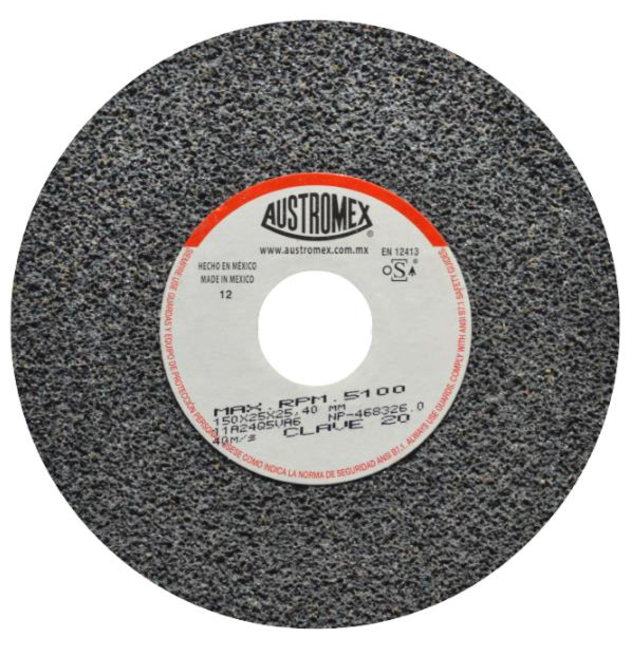
\includegraphics[width=7cm]{Figuras/a}
\caption{Piedra esmeril}
\label{fig:ECCI2}
\end{figure}

\begin{equation}
y(x_{i}) = a
\label{eq:cuadratica}
\end{equation}

En la Figura \ref{fig:ECCI} se observa el logo de la universidad ECCI.

\begin{figure}[htbp]
\centering

\includegraphics[width=3cm]{Figuras/LogoECCI}
\caption{Logo de la universidad ECCI}
\label{fig:ECCI}
\end{figure}

En la Tabla \ref{tab:ejemplo} se muestra el ejemplo de una tabla en Latex.

\begin{table}[htbp]
\centering
\caption{Ejemplo de una tabla en Latex}
\begin{tabular}{|c|c|c|c|c|}
\hline
A & B & C & D & E \\ \hline
 1 &   & 5  &   &   \\ \hline
  &   &  6 &   &   \\ \hline
  &   &   &   &   \\ \hline
\end{tabular}
\label{tab:ejemplo}
\end{table}

La Ecuaci�n \ref{eq:cuadratica} es utilizada para calcular los valores de $y$, a partir de los valores de $x$. \cite{oliveira2003relaccao}

\begin{equation}
y(x_{i}) = 4 + x_{i}^{2}-x^{\frac{a}{b}}
\label{eq:cuadratica}
\end{equation}

Programaci�n 2 es una disciplina de la universidad ECCI de tercer semestre
